%!TEX root = ../thesis.tex

\section{実験の概要}
作成した経路追従ソフトウェアを用いて実験を行う.
AIFormulaで実際に使われる会場であるAIモビリティパークで自律走行させて経路追従ソフトウェアの有効性を検証する.
なお, この実験では走行時間を短縮することを目的として徐々に並進速度を上げてパラメータチューニングをしながら実験を行う.
また, 使用するGNSS+IMUセンサ(VectorNav VN-200)には2通りの方位の補正がある.
それぞれ起動時に実行される地磁気の補正と一定時間5m/s以上で走行させた時に実行されるGNSSの補正があるが,
本実験ではGNSS+IMU(VectorNav VN-200)に対してGNSSの補正を実行した状態で行うこととする.
有効性を検証するために, いくつかの評価指標を設ける.

\begin{table}[H]
  \centering
  \caption{evaluation item}
  \begin{tabular}{cclll}
  \cline{1-1}
  評価項目                    &  &  &  &  \\
  \cline{1-2}
  走行速度(並進速度) {[}m/s{]}    &  &  &  &  \\
  走行時間 {[}s{]}            &  &  &  &  \\
  走行経路と目標経路の誤差の蓄積 {[}m{]} &  &  &  &  \\
  走行経路と目標経路の最大誤差 {[}m{]}  &  &  &  &  \\
  \multicolumn{1}{l}{}    &  &  &  &  \\
  \multicolumn{1}{l}{}    &  &  &  & 
  \end{tabular}
\end{table}

\section{実験環境}
本実験では茨城県常総市にあるAIモビリティパークにて行う.
Fig.6.1にAIモビリティパークの図を示す.

\begin{figure}[H]
  \centering
 \includegraphics[keepaspectratio, scale=0.1]
      {images/AerialViewAndMobilitysPerspetiveOfTheCourse.png}
 \caption{Aerial view and mobility perspective of the course}
 \label{fig:course}
\end{figure}

\section{実験装置}
本研究で使用する実験装置をFig.6.2に示す.
ハードウェアは, 本田技術研究所から貸与されたロボットを使用する.
このロボットは差動二輪+従動輪で構成された三輪モデルとなっている.
貸与された状態のロボットから従動輪をモータで駆動する形式に変更を加えている.
また, 安全面を考慮してロボットにアンテナを取り付けて遠隔で非常停止ボタンが押せるようにしている.
PCの仕様をTable.6.1に示す.
経路追従にはGNSS+IMUセンサ(VectorNav VN-200)を使用する.
ソフトウェアはROS 2を使用して構築している.

fig(センサに着目したロボットの画像)

本研究で開発した経路追従ソフトウェアは事前に用意した目標経路に沿って追従する動作を行う.
本実験で使用する目標経路は実験日と同日にAIモビリティパークを手動走行させて取得したGNSSデータを基準に作成している.
Fig.6.3に用意した目標経路をGoogle Map上にプロットした図を示す.

\begin{figure}[H]
  \centering
 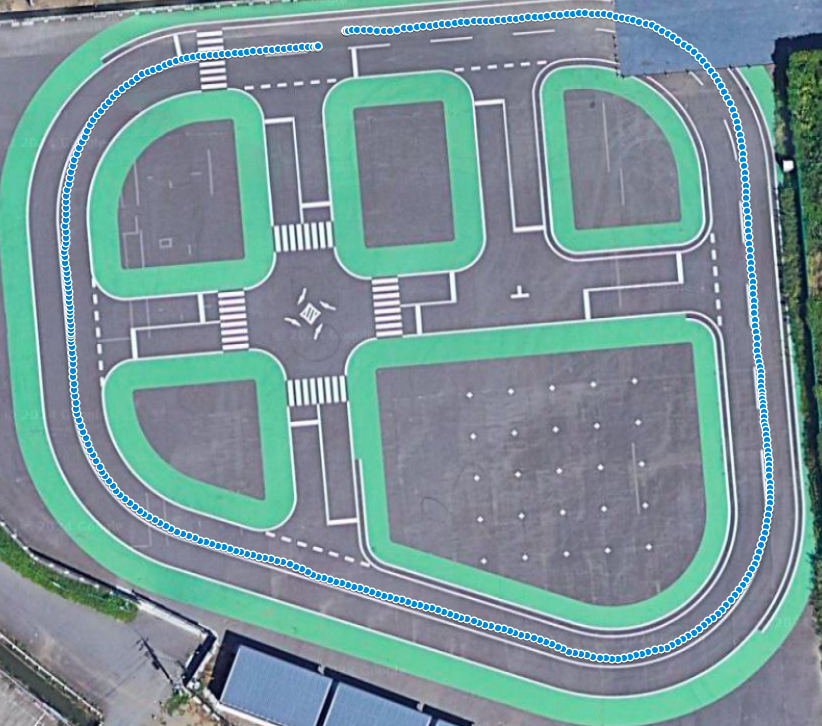
\includegraphics[keepaspectratio, scale=0.3]
      {images/targetpath.png}
 \caption{Aerial view and mobility perspective of the course}
 \label{fig:course}
\end{figure}

\section{実験内容}
AIモビリティパークで自律走行させることで経路追従の有効性を検証する.
並進速度は3m/sから開始させて, PIDゲインなどのパラメータを調整しながら徐々に並進速度を上げてパラメータチューニングを行った.
実験を行うコースをFig.6.4に示す.
ロボットはFig.6.4の丸で示された位置から矢印に沿うようなルートでコースを一周する.

\begin{figure}[H]
  \centering
 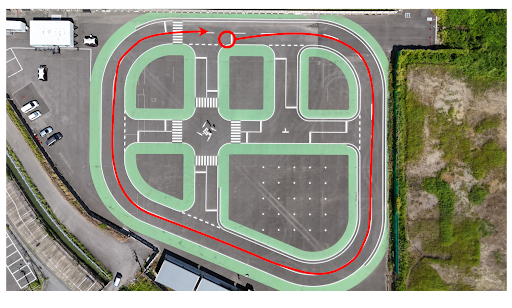
\includegraphics[keepaspectratio, scale=0.6]
      {images/AIFormulapath.png}
 \caption{Experiment path}
 \label{fig:path}
\end{figure}

\newpage

\section{実験結果と考察}

\subsection{実験1}
走行時のパラメータをTable.6.1に示す.
\begin{table}[H]
     \centering
     \caption{experiment1 parameters}
     \begin{tabular}{cclll}
     \multicolumn{1}{c|}{linear\_vel}     & 3.0  &  &  &  \\
     \multicolumn{1}{c|}{interval\_ms}    & 50   &  &  &  \\
     \multicolumn{1}{c|}{lookahead\_gain} & 1.0  &  &  &  \\
     \multicolumn{1}{c|}{p gain}          & 0.8  &  &  &  \\
     \multicolumn{1}{c|}{i gain}          & 0.0  &  &  &  \\
     \multicolumn{1}{c|}{d gain}          & 0.0 &  &  &  \\
     \multicolumn{1}{l}{}                 &      &  &  &  \\
     \multicolumn{1}{l}{}                 &      &  &  & 
     \end{tabular}
\end{table}

実験の結果, 並進速度3m/sでコースを一周することができた.
目標経路に対して大きなズレも無く追従することができることを確認できた.
実験時の走行経路と目標経路の軌跡をFig.6.5に示す.
また, 目標経路との誤差の遷移をFig.6.6に示す.
最後に評価項目の結果をTable.6.2に示す.

\begin{figure}[H]
     \centering
    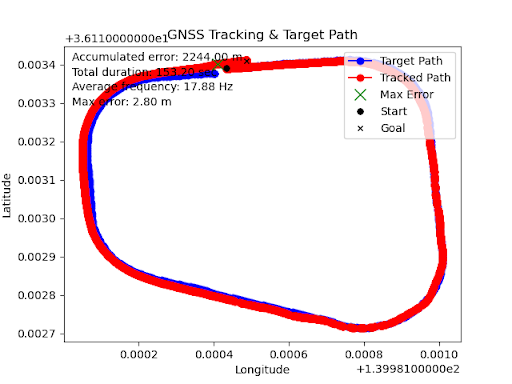
\includegraphics[keepaspectratio, scale=0.7]
         {images/3mspath.png}
    \caption{Trajectory of travel route and target route}
    \label{fig:path}
\end{figure}

\begin{figure}[H]
     \centering
    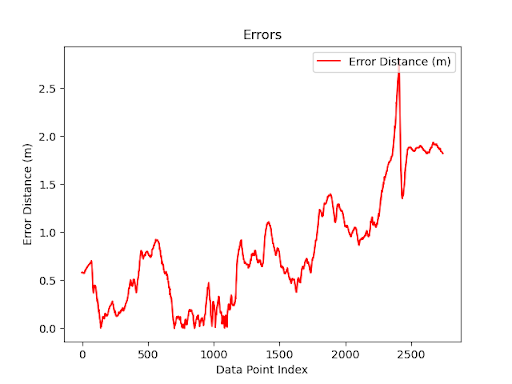
\includegraphics[keepaspectratio, scale=0.7]
         {images/3mserror.png}
    \caption{Transition of error from the target path}
    \label{fig:path}
\end{figure}

\begin{table}[H]
     \centering
     \caption{evaluation item}
     \begin{tabular}{cclll}
     \multicolumn{1}{c|}{並進速度{[}m/s{]}}         & 3.0  &  &  &  \\
     \multicolumn{1}{c|}{走行時間{[}s{]}}           & 140?   &  &  &  \\
     \multicolumn{1}{c|}{走行経路と目標経路の累積誤差{[}m{]}} & 2244.0 &  &  &  \\
     \multicolumn{1}{c|}{走行経路と目標経路の最大誤差{[}m{]}} & 2.8 &  &  &  \\
                                                &      &  &  &  \\
                                                &      &  &  &  \\
     \multicolumn{1}{l}{}                       &      &  &  &  \\
     \multicolumn{1}{l}{}                       &      &  &  & 
     \end{tabular}
\end{table}

\subsection{実験2}
走行時のパラメータをTable.6.3に示す.

\begin{table}[H]
     \centering
     \caption{experiment1 parameters}
     \begin{tabular}{cclll}
     \multicolumn{1}{c|}{linear\_vel}     & 6.0  &  &  &  \\
     \multicolumn{1}{c|}{interval\_ms}    & 50   &  &  &  \\
     \multicolumn{1}{c|}{lookahead\_gain} & 1.0  &  &  &  \\
     \multicolumn{1}{c|}{p gain}          & 1.0  &  &  &  \\
     \multicolumn{1}{c|}{i gain}          & 0.0  &  &  &  \\
     \multicolumn{1}{c|}{d gain}          & 0.15 &  &  &  \\
     \multicolumn{1}{l}{}                 &      &  &  &  \\
     \multicolumn{1}{l}{}                 &      &  &  & 
     \end{tabular}
\end{table}

実験の結果, 並進速度6m/sでコースを一周することができた.
コース東側の道で蛇行する動きを見せたものの, 経路から外れることなく周回することができた.
実験時の走行経路と目標経路の軌跡をFig.6.5に示す.
また, 目標経路との誤差の遷移をFig.6.6に示す.
最後に評価項目の結果をTable.6.4に示す.

\begin{figure}[H]
     \centering
    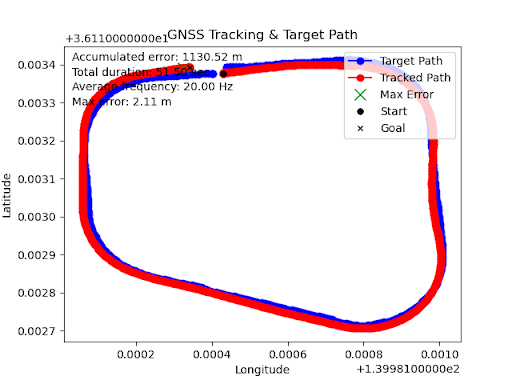
\includegraphics[keepaspectratio, scale=0.7]
         {images/6mspath2.png}
    \caption{Trajectory of travel route and target route}
    \label{fig:path}
\end{figure}

\begin{figure}[H]
     \centering
    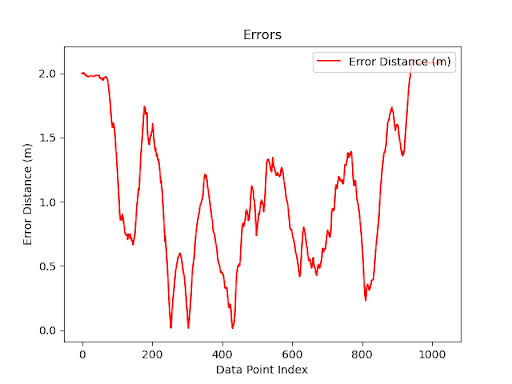
\includegraphics[keepaspectratio, scale=0.7]
         {images/6mserror.png}
    \caption{Transition of error from the target path}
    \label{fig:path}
\end{figure}

\begin{table}[H]
     \centering
     \caption{evaluation item}
     \begin{tabular}{cclll}
     \multicolumn{1}{c|}{並進速度{[}m/s{]}}         & 6.0  &  &  &  \\
     \multicolumn{1}{c|}{走行時間{[}s{]}}           & 43   &  &  &  \\
     \multicolumn{1}{c|}{走行経路と目標経路の累積誤差{[}m{]}} & 1130.0 &  &  &  \\
     \multicolumn{1}{c|}{走行経路と目標経路の最大誤差{[}m{]}} & 2.11 &  &  &  \\
                                                &      &  &  &  \\
                                                &      &  &  &  \\
     \multicolumn{1}{l}{}                       &      &  &  &  \\
     \multicolumn{1}{l}{}                       &      &  &  & 
     \end{tabular}
\end{table}